\documentclass{business}
\usepackage[margin=1in]{geometry}
\usepackage{hyperref}
\usepackage{float}
\usepackage{longtable}
\usepackage{csvsimple}
\usepackage{fontspec}
\setmainfont{CMU Sans Serif}
\business{Prep-U Tutoring Service}
\names{Edouard Des Parois Perrault and Arthur Huang}
\school{Lower Canada College}
\eventyear{2021-02}
\city{Montreal, Quebec, Canada}
\event{Business Plan}
\logo{./images/prep-u-logo.png}
\logoscale{1}
\begin{document}
    \maketitle
    \tableofcontents
    \newpage
    \section{Executive Summary}
    Prep-U is an innovate online tutoring service. Prep-U leverages the online VoIP communication platform Discord in order to provide academic support to students. Prep-U is also highly profitable, and has no startup costs, as the founders have identified several areas in which prices can be cut without affecting the overall quality of the education provided by the service. Therefore, not only is Prep-U almost certain to generate a sizable return on investment, but it also features a much more affordable pricing model than its competitors in the online education industry. Moreover, the founders themselves are high school students, and have considerable experience offering academic help to their peers. They have a passion for education and wish to make use of novel high-tech solutions in order to make academic support more flexible, more fun, and more engaging for students. The pandemic has presented a unique challenge for many, and students are no exception. In difficult times such as these, the founders hope to provide assistance in an accessible way. All in all, the founders of Prep-U designed this modern and affordable business with the company slogan in mind; the prep \emph{you} need to succeed.
    \section{Company Description}
    \subsection{Overview}
    Prep-U Tutoring is an online service that allows students to obtain help with their assignment online. Prep-U offers help in all high school subjects, such as mathematics and science. Prep-U uses the social platform Discord to deliver its academic services. This enables Prep-U Tutoring to keep its prices much lower than its competitors, most of whom have proprietary systems of their own.
    \subsection{Location}
    The company, being an LCC, will be registered in Montreal, Quebec, Canada. Prep-U, however, has no physical office space as it will operate solely online. Moreover, Discord is a platform that can be customized and used free of charge. Therefore, there are no charges associated with physical office spaces. 
    \subsection{Legal Structure}
    The founders of Prep-U have decided to make their company a Limited Liability Corporation. The founders decided that this option suits their needs the most as it offers them more protection. Prep-U is a service through which the founders tutor multiple individuals each day (see Section \ref{operations}). In the unlikely case that any one of these individuals blames Prep-U for their failures, they might file a lawsuit against the company, but cannot do so against the founders themselves. Moreover, if this venture turns out to be unprofitable, it will be considered a separate entity, and therefore will go bankrupt without the founders being affected personally. The only downside to an LLC is the price of the incorporation paperwork, though the founders believe that this price is justified by the aforesaid advantages.
    \subsection{Organization}
    Prep-U makes use of the platform `Discord' due to its advantages over other solutions (see Section \ref{choice-of-platform}). We will create a virtual Discord \textbf{server}, which we will use as our platform. Discord servers are made up of \textbf{channels}, which are similar to rooms in an office. There are \textbf{voice channels} and \textbf{text channels}. Voice channels are used for presentations and tutoring sessions while text channels are places where the students can ask questions. The founders act as head tutors and tutor in voice channels. They also answer the questions submitted in text channels. As Prep-U expands, more tutors will be hired (see Section \ref{operations} and Section \ref{long-term}). 
    \subsection{Educational Philosophy}\label{educational-philosophy}
    Prep-U is committed to raising the standard of online education by putting modern theories into application. As shown in Section \ref{pillars}, the founders have identified a selection of five pillars that they believe define a successful venture in the online education industry. Throughout this report, the founders will demonstrate how Prep-U achieves each of these pillars. \par
    An example of the modern education theories the founders seek to put into application in the context of their virtual classrooms is \textbf{learning objects}. Learning objects are digital artifacts employed to make lessons more interactive for students. Prep-U’s position as an online service allows it to easily leverage these concepts. \cite{Vanessa} Prep-U is determined to show how online education has incredible potential to make the experience more interactive and more enjoyable for students. Prep-U demonstrates, during its sessions and lessons, that it’s possible for students to create a different type of connection with their educator. As researcher Aaron Doering puts it, in online classrooms, ``traditional hierarchical classroom roles are blurred.'' \cite{Doering2007} Prep-U thrives despite being online, for it is a collaborative effort in lieu of an individual pursuit. Prep-U is more than just shadow education, it’s a discussion. Prep-U hopes to inspire its students and to transmit them the joy of knowledge so that they can communicate it to their peers and attract additional customers. The founders understand that not all students appreciate learning, but believe that online education can drastically contribute in alleviating such unjustified disgust and making such an important part of the students’ lives enjoyable. Moreover, educational philosophy is reflected in the educators, for they are the ones who ultimately apply these principles. As such, Prep-U has a rigorous employee hiring program. It also takes any complaints towards its staff or community very seriously (see Section \ref{operations}).
    \section{Industry Analysis}\label{industry-analysis}
    The online education industry has experienced exponential growth rates in the past few decades. Online higher education courses have nearly tripled between 1995 and 2003. \cite{Wiest2012} The value of the web-based training industry as a whole grew from \$550 million in 1998 to \$11.4 billion in 2003. \cite{Singh2004} Further, the private tutoring industry is growing rapidly in Canada, with many new private tutoring businesses making an appearance. \cite{Davies} The market for private tutoring as a whole is expected to reach US\$218 billion by the year 2027. \cite{Private2020} The market for test preparation alone is expected to grow by 10.72 billion dollars during 2020-2024, which represents a CAGR of 6\%. \cite{TestPrep2020} This trend is further stimulated by the pandemic. Covid-19 has had a positive effect on the online tutoring service industry, and there is considerable evidence suggesting that parents are more likely to hire private tutors in light of the current situation. The CEO of Cisco went so far as to state that ``education over the Internet is so big, it is going to make email look like a rounding error.''\par
    Prep-U is specifically targeting the after school high school tutoring industry (see Section \ref{target-market}), known as \textbf{shadow education} \cite{Zhang}. This industry has followed the same trend as the global online education industry, and is expected to follow a CAGR (Compound Annual Growth Rate) of 16.1\% from 2020 to 2027. \cite{Online2020} 
    \begin{figure}[H]
        \centering
        \caption{Industry analysis of the global online tutoring industry. \cite{Global2019}}
        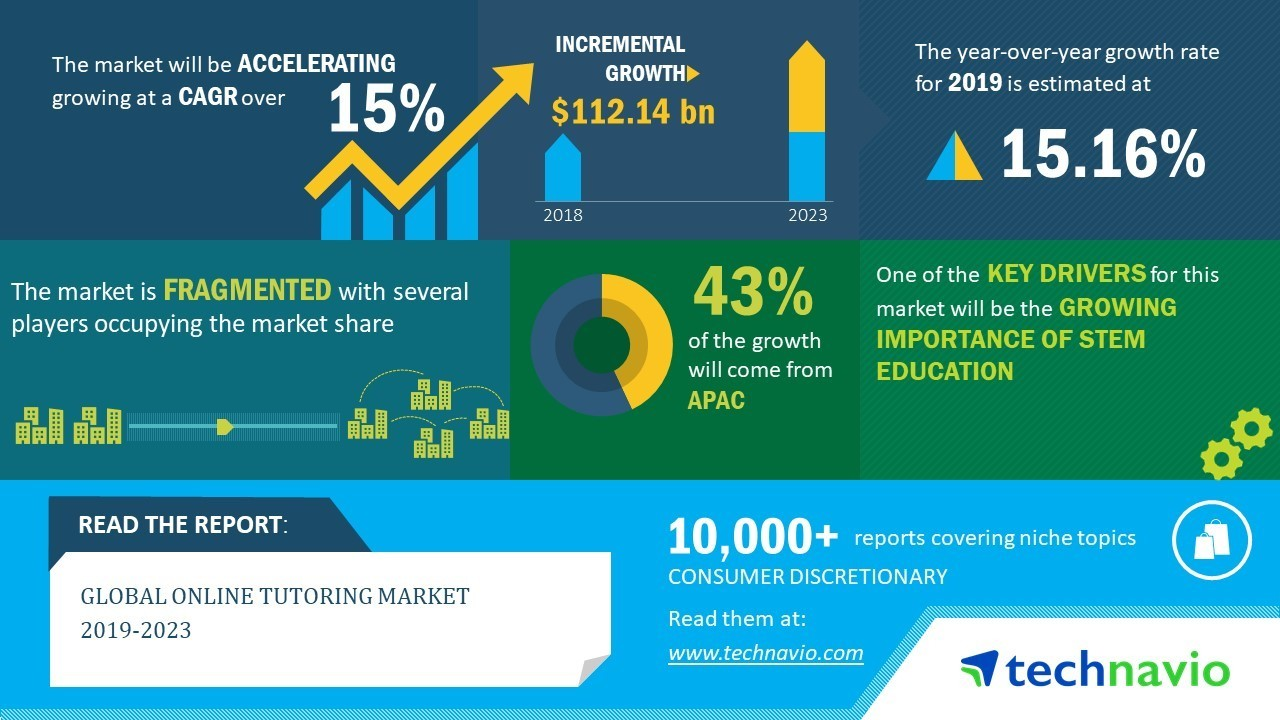
\includegraphics[scale=0.3]{./images/infographic-1.jpg}
    \end{figure}
    \begin{figure}[H]
        \centering
        \caption{Impact analysis of COVID-19 on the online tutoring industry. \cite{K-12-2020}}
        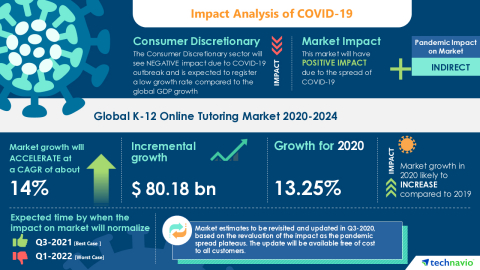
\includegraphics[scale=0.8]{images/infographic-2.jpg}
    \end{figure}
    \section{Target Market}\label{target-market}
    Prep-U exclusively targets high school students. There are four reasons for this. First, the founders seek to target a specific sector of the market  in order to maximize efficiency and effectiveness. Second, restricting the market to high-school students ensures that Prep-U can keep up with advances in the industry; especially in an emerging field (see Section \ref{industry-analysis}), additional developments are bound to be made as more research becomes available. It is easier for the founders to keep up to date with this research if the scope of the industry is kept smaller. Third, since Prep-U does not employ traditional means of advertising, it must establish a good reputation (see Section \ref{marketing-and-sales}). Limiting the size of the market ensures that it can excel in this particular field. Lastly, since the founders are themselves high school students, they are certain about the demand for online tutoring. The founders have been conducting a pilot project of their own within their school, and have seen considerable demand for the service. The founders are sure that growth can be expected in a high-school environment.\par
    The founders classify their tutees into three categories, although some may be part of many categories at a time. 
    \subsection{Category A}
    The first category is made up of students who have fallen behind in their work in the transition to online school. The pandemic has prompted many high schools to transition online, and evidence suggests that students are not accustomed with this new online system, and therefore falling behind and struggling to succeed. In short, the drastic paradigm shift has proven to be nefarious. Hence, students in this situation reach out to Prep-U in order to obtain support. 
    \subsection{Category B}
    The second category of students turns to online education \emph{voluntarily} in order to replace their current in-person–––or perhaps even online––tutoring organization, either because Prep-U offers better service, is more convenient, or because of its lower price. Students may prefer online tutoring for several reasons. First, they may enjoy it because it is much more convenient than organizing physical meetings. Second, they may prefer it because they have less difficulty interacting with their teacher online. Although the efficiency of online education in the context of large class sizes may be questionable, the founders have noted that many students find it easier to interact one-on-one with a teacher online than in person. 
    \subsection{Category C}
    The third category of students reflects an increase in demand for education credentials. Professor Scott Davies of McMaster University argues, in his paper \emph{School Choice by Default}~\cite{Davies}, that competition for credentials and access to selective higher education institutions is increasing. As a result, this has added extra pressure on students to partake in rigorous academics. Hence, parents have begun to seek all opportunities they can to allow their children to obtain these coveted credentials and enroll in selective programs. Some parents have opted to send their progeny to private institutions, though the price-tag of such institutions is not always within the budget of these families. The next best option is therefore to seek shadow education online, which is where Prep-U comes in. In short, this category is made up of families who seek to give their children good education for an affordable price.
    \section{Competitive Analysis}
    The significant increase in popularity of e-learning (see Section \ref{industry-analysis}) has prompted many novel entities to enter the market in order to offer a similar service. The founders have identified two primary categories of potential competitors; online and physical.
    \subsection{Online}
    Online competitors include institutions such as Varsity Tutors, Chegg, and The Princeton Review. Essentially, they are the online branches of any such company. One of the major advantages of online education is the lack of real-estate costs. In the case of this category however, these costs are instead invested in proprietary digital systems, which are tailored to the specific needs of the particular institution. As a student of The Princeton Review, Edouard can attest to the advantages of these systems. However, proprietary systems also offer significant disadvantages. For one, technical difficulties and small bugs are commonplace, and maintaining them is troublesome. As a hobbyist software developer, Edouard appreciates the complexity of such systems and recognizes that bugs are impossible to avoid, though this does not make them any more tolerable. Professionals––who are not necessarily familiar with education––must be employed to support and address any technical glitches, which leads to the next disadvantage; proprietary systems are expensive to develop, and drive prices upward. These institutions charge on average \$20 an hour for one-on-one tutoring. In addition, some services, such as SAT preparatory evaluations, can cost as much as \$1500.
    \subsection{Physical}\label{phsyical-competition}
    The second potential source of competition is physical competition. This includes institutions, such as Prep Academy, that have tutors who visit the student in person. One of the major disadvantages of physical tutoring is that it is not on demand. Online organizations tend to pride themselves in offering 24/7 support, as it is possible for them to outsource their tutors to other time zones. Moreover, additional costs are necessary for physical office spaces, and more time must be allocated to the tutor for transportation. Hence, its service area is severely limited. In order to address this problem, tutoring agencies that offer in-person classes tend to have multiple chapters in several provinces or states, which creates a significant amount of bureaucracy and its related costs.
    \subsection{Other}
    Although the founders recognize that some universities offer online programs, the founders do not consider these potential competitors, as they do not fall in the scope of the industry (see Target Market). Moreover, the founders also recognizes that some institutions fall into both of the aforesaid categories, as is the case with The Princeton Review. Finally, the founders are also aware that not all tutoring is done in person, and that some tutoring agencies allow students to collaborate and form classrooms of their own. The founders also attempt to simulate such an environment in an online fashion (see Section \ref{educational-philosophy}).
    \subsection{Strengths}
    Prep-U's primary objective is to offer quality education while remaining in the range of the budget of its target market (see Section \ref{target-market}). A significant advantage of Prep-U over competitors is that Prep-U charges a monthly subscription in lieu of an hourly rate. Students benefit from using the platform more, not less. Moreover, instead of charging hourly rates in the neighborhood of \$20 per hour, Prep-U charges \$10 per month, without any additional fees. The choice of a cheap and affordable platform on which to deploy the service is what makes these savings possible (see Operations).
    \subsection{Weaknesses}
    The platform that was selected, however, was not originally designed for education (see Choice of Platform). This makes it not completely compatible with this venture. Although, thanks to the platform, it \emph{is} possible to upload files, to send text, and to send emoticons, it is \emph{not} possible to send formatted mathematical and chemistry equations. This is a significant disadvantage that can only be solved by using a proprietary platform. Unfortunately, using Prep-U, students will be forced to upload images of their work if they want to use complex equations, and tutors will be forced to reply with images as well.\par
    Moreover, Discord also does not come with tools for tutors to use when teaching. When presenting to their tutees, tutors must use separate software, such as Google Jamboard or Microsoft Paint. The availability of such software free of charge, however, lessens the impact of this problem. Prep-U does not impose any software to its tutors, so long as the company gets positive feedback from students. Screen recordings must also be done through separate software, as this cannot be done via Discord. Prep-U officially recommends OBS to its tutors on Windows, and Quicktime on Mac. This variety in software can make it logistically more complex for the founders to manage their tutors, though this will only realistically become a problem when new staff is hired (see Future Vision).
    \subsection{Barriers of Entry}
    There are comparatively few barriers of entry into this industry. Whereas physical tutoring has significant logistic challenges (see Section \ref{phsyical-competition}), these challenges are not present in the context of online education. In her introduction to professor Kaye Shelton’s book \emph{An Administrator’s Guide to Online Education}, Rena M. Palloff, the owner of the reputable educational company Crossroads West, warns against a dangerous tenet she believes permeates the educational field. She is convinced that a large number of individuals believe that online education is easier to organize and deliver than in-person education due to the lack of such brick-and-mortar costs. She believes that it is this erroneous belief that often prompts many to begin their own private tutoring organizations. The author argues, however, that this belief is untrue, and often results in failure. \cite{Shelton2005} Teaching online is just as complex as teaching in person. If not, it presents even more challenges, as educators must sustain the interest of a class through a screen. The biggest barrier in this industry is not starting up, it is maintaining the service. The founders believe that they have the tools to overcome these barriers as they already have experience in the industry, and understand the complexities of starting such a business.
    \section{Marketing Plan and Sales Strategy}\label{marketing-and-sales}
    Prep-U will not make use of any official form of advertising whatsoever. The business does not, for instance, purchase ads on Facebook or Instagram. The founders made this decision in order to ensure that startup and operation costs are kept as low as possible. Moreover, the founders do not want the business to be a victim of its success and to grow too rapidly. Instead, Prep-U predominantly relies on word-of-mouth. Hence, most of the marketing is embedded in the practices of the organization itself.
    \subsection{Reputation}
    Prep-U’s only product is knowledge. Thus, Prep-U must maintain a good reputation in the way it transmits this knowledge to ensure that it is able to rely on word-of-mouth for advertising. As such, Prep Tutoring is committed to raising the standard of online education by putting modern education theories into application (see Section \ref{educational-philosophy}). 
    \subsection{Choice of Platform}\label{choice-of-platform}
    The choice of the platform is in itself a marketing decision. Discord has several advantages over other platforms. First, the founders have heard many students complaining that platforms such as Slack or Microsoft Teams are too complex and too formal for their liking. While these may be popular solutions for businesses, students do not enjoy them. The founders wish to make sure that their platform is best suited for their students, preferably something students already use. Although Discord does not collect data on the age of its users, and therefore cannot determine for sure whether it is frequently used by high schoolers, the company CEO himself has speculated that most of his user-base, made up of 250 million registered users, \cite{Sherr2019} belongs to this demographic. Eros Resmini, an angel investor for Discord, has admitted that “I’m really cool when I wear my Discord T-shirt when I’m in high school.” \cite{Jargon2019} Because many students are already familiar with the platform, it will not be necessary for them to learn new software. The founders believe that the accessibility of educational platforms is a major selling point. High-school students primarily use Discord to create gaming communities. Using Discord for education may therefore aid in creating a collaborative environment. Finally, the platform also has an extremely intuitive user interface (see Operations), which will attract students. Long story short, Prep-U’s usage of Discord is unique, and students will surely enjoy using it. 
    \subsection{Social Media}
    One of the major avenues form Prep-U, in addition to word-of-mouth, is social media. The founders, however, have no intention to invest in social media ads, for they are too expensive. Instead, the founders prioritize giving the business a strong social media presence; Prep-U has an extremely active Instagram account, and runs weekly events such as the Question of Week. Every week, Pace posts a difficult question on its social media story. This question is heavily inspired from one or several of the questions that were submitted and answered throughout the course of that particular week.
    \section{Operations}\label{operations}
    \subsection{Opening Hours}
    The founders are unable to consecrate all of their time to Prep-U by virtue of their education. In practice, this should not be too much of an issue, as most Prep-U’s students also go to school during that time, as the target area is North America. In other words, from about 8:00 am to 5:00 pm every week day, there is significantly less demand for the service.
    \subsection{Discord Server}
    The platform is a Discord \textbf{server}. Discord servers have several different \textbf{channels} that can be given purposes. All communication, and hence all activity on the server, is done through such channels. In addition, the server can be configured with \textbf{bots}, which may be referred to as plugins, to give it additional functionality. In addition, \textbf{roles} can be given to students, either manually by the administrator or automatically through a bot. Roles can be seen as permissions, and can limit the ability of a student to interact with a given channel. Limitations can vary, from preventing a user from seeing the channel altogether to simply making it impossible for them to submit messages of their own. Channels can be grouped into groups, which help with organization.
    \subsection{Subjects}\label{subject-channels}
    Each subject has a total of five channels. These channels are grouped under a group with the name of the subject. Each subject has the following channels.\par
    \begin{minipage}{0.5\textwidth}
        \begin{itemize}
            \item A \textbf{voice channel} for audio-visual presentations
            \item An \textbf{announcement channel} for important notices. Such notices mainly include dates for presentations.
            \item A \textbf{question channel} where students can submit questions.
            \item A \textbf{resources} channel, where tutors can post resources that are of relevance to all students in that course. For instance, the digital whiteboards for the presentations are posted in resources.
            \item A \textbf{chat} channel, where students can talk amongst themselves. This is to encourage communication and a sense of community.
        \end{itemize}
    \end{minipage}
    \begin{minipage}{0.5\textwidth}
        \centering
        \begin{figure}[H]
            \centering
            \caption{A subject channel}
            
\includegraphics[scale=0.8]{./images/server-subject.png}
        \end{figure}
    \end{minipage}
    The example given in the image is math. However, in practice, this is too general. Subject names will have a level of detail similar to `Grade 10 Enriched Math' to ensure that everything remains organized and adequate to the level of the students involved. This also means students must declare their level when they register for the service. The server is configured so that. Special permissions are given to students so that they are only able to see subjects that are of relevance to them. 
    \subsection{Moderation}\label{moderation}
    In servers with large amounts of members such as this one, it is important to ensure that conversations remain friendly. The reputation of Prep-U is extremely important (see Section \ref{marketing-and-sales}), and the founders ensure that text channels remain clear of any sign of violence or hateful behavior. To keep costs low, an additional tutor will only be employed to complete this task once Prep-U has grown substantially in size (see Future Vision).
    \subsection{Other Channels}
    In addition to the channels mentioned in Section \ref{subject-channels}, the server has several channels that are not part of a particular subject. These channels are in the `general' group and are visible to all students at all times.
    \begin{itemize}
        \item A channel called welcome to greet newcomers to the server.
        \item A rules channel where we post all rules for the server. This is also where the Code of Conduct is available for all users to see. Prep-U reserves the right to ban any student that repeatedly infringes this code of conduct.
        \item A subjects channel where students can select the subjects they want to see. This has no effect on billing, but allows them to keep the server organized. There is no reason for a student to get notifications for a course they are not taking.
        \item An announcements channel, where students can find server-wide announcements.
        \item A channel called General where students from all courses can talk, so long as it is respectful conversation.
        \item The feedback channel is where students can submit complaints against the staff if they have any. Due to the importance of reputation, Prep-U takes this feedback very seriously. Complaints are confidential and anonymous.
        \item The testimonial channel is where students can leave small reviews. These reviews may be used for promotional reasons.
        \item The premium channel is where users can purchase a premium subscription to the service.
    \end{itemize}
    \begin{figure}[H]
        \centering
        \caption{General channels}
        
\includegraphics[scale=0.5]{images/general-channels-2.png}
    \end{figure}
    \subsection{Registration}\label{registration}
    If a student seeks to obtain a premium subscription to this service, which allows them to access more tutoring sessions and to ask questions in the chat, they do so via the \textbf{premium} channel. A bot watches over the channel and processes payments via PayPal in a confidential manner. Prep-U charges \$10 per month, without any additional fees.
    \subsection{Tutoring Sessions}
    There are three tutoring sessions every week. One on Monday, one on Wednesday, and one on Saturday. The sessions are spread out to accommodate as many schedules as possible. They take place in the evening at 7 to allow students to get started on their homework or attend any co-curriculars they may have. Tutoring sessions are subject-specific.\par
    The schedule is not set in stone. Hence, depending on the demand for the service, additional sessions may be scheduled. The time and date of these sessions is determined on a case-by-case basis by communicating with the students. For instance, closer to exam periods, additional sessions are scheduled depending on the availability of students and tutors.\par
    Sessions take place using the Discord voice channels, as shown in Figure \ref{teacher-vc}. Each subject has a voice channel for this purpose (see Section \ref{subject-channels}). Special permissions for the server allow the founders to prevent anyone from speaking but the tutor responsible for the session. In addition, the tutor can share their screen, and can prevent other students from sharing theirs.
    \begin{figure}[H]
        \centering
        \caption{A Voice Channel with one Participant}
        \label{teacher-vc}
        
\includegraphics[scale=0.5]{images/teacher-vc.jpg}
    \end{figure}
    The restrictions on the vocal participation of the students is to prevent chaos from emerging during a session. Despite the restrictions and voice, questions are still encouraged. Students with paid accounts get a special feature––they can ask questions in a text channel, as shown in Figure \ref{ask-question}.
    \begin{figure}[H]
        \centering
        \caption{A student asking a question}
        \label{ask-question}
        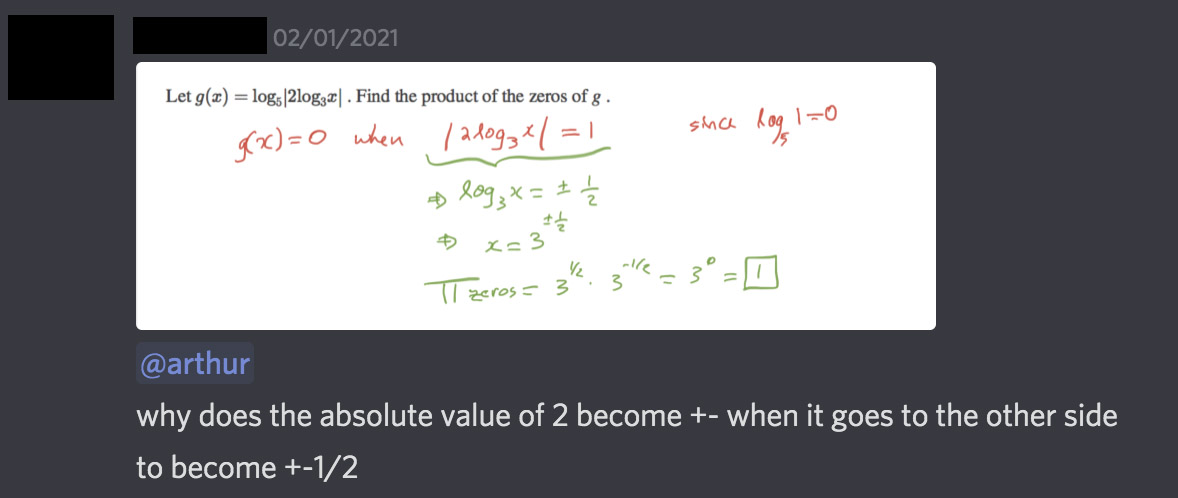
\includegraphics[scale=0.3]{images/ask-question.jpg}
    \end{figure}
    Additional bots and configuration can be made to ensure that these text channels stay organized. Students can send images of problems they may encounter. They can also add text to support their query.\par
    A tutoring session has 45 minutes of planned content and 15 minutes of answering questions. The planned content in question depends on subjects that have been on demand over the course of that week. The founders carefully monitor the questions that are asked by the students in order to create pertinent sessions. All sessions are, of course, optional.\par
    The subjects of these sessions are largely dependent on the demand for the days leading up to the meeting. Hence, some sessions may be of little relevance to certain students. Students are not at all expected to attend each session, and if demand is too low, the schedule––and perhaps the operation as a whole––may be revised.\par
    \subsection{Questions}
    The platform also allows students to submit questions in a text channel destined for this purpose. All text channels are moderated to ensure that all conversations are appropriate (see Section \ref{moderation}). This is just as much to keep the server organized as it is to prevent bullying and undesired behavior. Automation is put in place to ensure that any question submitted is added to a database of unanswered questions. Tutors are then able to answer these questions.\par
    The founders will begin by being the only tutors on the platform. As Prep-U grows in size, more tutors may be necessary. Questions can be answered at any time, so long as they are answered in less than 10 minutes during the \textbf{Q\&A windows}. These windows are every day of the week from five pm to 12 pm. After that point, questions may or may not be answered before the next available window. During the weekend, the windows depend on the availability of tutors, and are posted on the \textbf{server-announcements} channel. \par
    At first, it will be impossible for the founders to cover more than these two windows. As more tutors join the team, they may be extended. Tutors may be given ratings for their answers by students. Students rate them from 1 star to 5 stars. As the reputation of Prep-U is of great importance (see Section \ref{marketing-and-sales}), tutors with ratings below four stars are called and questioned by the founders. In addition, they may be suspended. Students may add more information about why they have  awarded a specific rating. The founders are open to any criticism, and can be directly contacted by the students. The pricing model of tutors is discussed in greater detail in the next section.\par
    Answering questions is one of the main advantages of Prep-U. There is considerable flexibility in terms of when the questions are answered, so long as during the windows, they are answered within 10 minutes. The founders moderate this to ensure that this is respected. The quality of the answers is one of the priorities of Prep-U, and tutors are expected to provide good answers. 
    \subsection{One on One}
    Prep-U also offers one-on-one tutoring sessions. Students can send  a message to a special text channel destined for this purpose. Then, an available tutor will be allocated to that student. Students must also submit something which they want to talk about. These requests are processed by the founders, who determine how long an answer to this question will take and who is best suited for the role. Some automation may work into this process.\par
    Prep-U is dedicated to ensuring that there are no additional fees apart from the monthly fee. A student may reserve a maximum of two one-on-one sessions, each of a maximum of 30 minutes. If a student exceeds the time limit, they are encouraged to continue the discussion over text.\par
    Students may not pay extra to get more time. The monthly fee is the only price they are allowed to pay. The reason for this is marketing––the founders do not want Prep-U to give the impression of being some sort of overly capitalistic despot.
    \subsection{Public Sessions}
    An extra session on Friday will be open to the public. This session is more flexible, and is during a time that is less popular for students. The topics of public sessions tend to be more general, and are more for marketing reasons than anything else. Guests are not allowed to ask questions of their own, but because Prep-U believes in the importance of open source, a large amount of previously answered questions can be viewed free of charge. 
    \section{Management and Organization}
    \subsection{Employees}
    The people in charge of Prep-U Tutoring will be the founders, both serving as head tutors. The moderation team will start out with just the head tutors, with moderators hired if Prep-U experiences significant growth. Additional tutors will also be hired according to the growth of the business.
    \subsection{Compensation}
    The moderation team will be compensated based on a contract negotiated in advance. Contracts are negotiated on a case-by-case basis. Tutors, on the other hand, will will split the profits with the owners based on how much they tutor. This is negotiated on a case-by-case basis with the tutor. This implies that hours must be reported to Prep-U. Any unreported hours will be considered nonexistent. Moreover, a rigorous interview process is completed to ensure that the tutor will be a meaningful member of the Prep-U community.  Prep-U does not offer any full-time employment, though during busy times of the year, it is possible that some tutors may have the opportunity to work longer if they so desire. Prep-U does not offer any incentives of any kind, apart from its flexible working hours. 
    \section{Long-Term Development}\label{long-term}
    Prep-U will be developed in two stages. Each stage is outlined below.
    \subsection{Stage 1}\label{stage-1}
    The first stage is the startup stage. During the first stage, the only platform used is Discord. Moreover, Prep-U only has two employees––the founders––who have the roles of the Head Tutors. This stage will be in effect as the server has 0 to 1000 paying members. All payment is done through Discord integrations (see Section \ref{registration}). Because the only two employees are the founders, there is virtually \textbf{no risk} associated with this stage, as it is not possible for Prep-U to go bankrupt without having spent any capital. The only resource the founder must spend to get off the ground is their time.
    \subsection{Stage 2}
    The second stage is put in effect once the server exceeds 1000 paying users. At this point, special negotiation will need to be done with Discord in order to get better server quality in order to sustain this amount of users. This will represent an additional expense for the business. Moreover, a website will be created in order to offer better payment processing and better advertising. This will also represent an additional liability for the business. Fortunately, these liabilities do not need to be covered by loans, as Prep-U can rely on its savings from Stage 1.
    \section{Financials}
    Prep-U will make use of the GAAP standard for its accounting practices. Financial projections for the first 6 months can be found in Table \ref{financial-projections}\par
    \begin{table}[H]
        \caption{Future Financial Projections}
        \label{financial-projections}
        \csvautotabular{./data/financial-projections.csv}
    \end{table}
    In Table \ref{financial-projections}, we assumed a relatively constant growth, with the most significant growth taking place at the beginning of the business. The total revenue increases at a constant rate, and is not subject to any deduction whatsoever, for the business will not incur any such expenses during stage one of its development (see Section \ref{stage-1}). The founders have a assumed that a conservatively small fraction of the users with an account will sign up for premium. In reality, however, the founders hope that a larger fraction of users will sign up for premium, yielding a larger revenue. The founders believe that users without a premium subscription will quickly find the service to be rather useful and will be enticed to purchase premium.\par
    Assuming the founders are working about 4 hours per week, in the six months covered in Table \ref{financial-projections}, the are paid about \$13 per hour each. This is a rather conservative measure, and the founders hope to beat these predictions and experience even more significant growth.
    \section{Appendix}
    \subsection{Pillars of the Business}\label{pillars}
    The founders, after having conducted research in this regard, have come up with a list of five keys to success when it comes to an educational venture. \cite{Sun2016}. Thought this report, the founders adhere to these pillars. \par
    \begin{enumerate}
        \renewcommand{\theenumi}{(\Roman{enumi})}
        \item Well-designed course content;
        \item Motivated interaction between the instructor and learners;
        \item Well-prepared and fully-supported instructors;
        \item A creation of a sense of online learning community; 
        \item A rapid advancement of technology.
    \end{enumerate}
    \subsection{Licenses}
    According to research conducted by the founders, There is no need for a license in order to provide this service in Canada.
    \newpage
    \bibliographystyle{IEEEtran}
    \bibliography{refs}
\end{document}